\graphicspath{{Chapters/SCT/Figures/}}

\chapter{SCT Temperature Monitoring}
%\chapter{ATLAS Semiconductor Tracker Temperature Monitoring}
\label{chap:SCT}

\section{Introduction}

In order to mitigate the effects of radiation damage, it is necessary to
maintain the SCT modules at a temperature of approximately $-7^{\circ}$C. The
SCT and Pixel sub-detectors use a common evaporative cooling system to keep
their silicon modules at the required temperatures. Monitoring of the module
temperature is important to ensure that the cooling system is functioning as
designed and that the modules are still coupled to the cooling structures.
Additionally, monitoring of the temperature difference between the front and the
back of barrel modules provides a check of the mechanical integrity of the
modules. This
chapter describes tools developed to monitor variables associated with the
temperatures of SCT modules, and presents results for twenty-two months of
operation between January 2010 and October 2012.

%An overview These are described in this section, along with results for
%twenty-two months of operation between January 2010 and October 2012. 

%An
%overview of the Inner-Detector cooling system is given in
%Section~\ref{sec:SCT-CoolingDesc}.
%An overview of the
%Semiconductor Tracker (SCT) was given in
%Section~\ref{sec:Detector-SCT}. 

\subsection{Effects of Radiation Damage on Semiconductor detectors}
Given the LHC design luminosity of $10^{34}$cm$^{-2}$s$^{-1}$, the
inner layers of the 
SCT are expected to receive a radiation dose of up to
$2\times10^{14}\rm{n_{eq}/cm}^2$~\cite{Ahmad200798} over the course of its design
lifetime of 10 years.
Exposure to such high radiation doses causes damage to the silicon detectors. 

The primary method
of radiation damage is interactions with irradiating particles displacing nuclei from
their lattice position, damaging the structure of the material. Displaced nuclei
form stable defects in the material, and act as acceptors, changing the
effective doping of the material. Exposure to radiation will cause an n-type
semi-conductor to become more p-type, and will eventually change the
material from n-type to p-type, in an effect known as \intro{type-inversion}.
The change in effective doping has two
effects: a loss of mobility of drifting electrons and ions due to recombination, and an increase in
the leakage current across the junction. This leads to lower charge collection
efficiency and increased noise. If the radiation damage is now too great, charge
collection efficiency maintained by increasing the displacement voltage, though for sufficiently high radiation doses it
becomes impossible to fully deplete the detector. It is therefore essential to
reduce the effects of radiation damage as much as possible.
 
%The effects of exposure to radiation have both
%an immediate and a prolonged effect. Immediate effects include the removal of
%donor nuclei from the lattices, and creation of acceptor like defects. Due to the
%complicated kinetics of these defects after the radiation, after type inversion
%has occurred an annealing effect
%occurs which initially reduces the number of acceptor-like defects, on a timescale of
%approximately two days, but on a longer term a `reverse annealing' occurs,
%increasing the number of acceptors. The rate of the reverse annealing effect is dependant on the temperate of the
%silicon. It is found that for temperatures of approximately -7$^{\circ}$C the
%reverse-annealing effect is effectively frozen out~\cite{Lindstrom2001308}. Since the reverse annealing
%occurs even after radiation, it is important to run the detector cooling at all
%times, not just when particle collisions are occurring.

It is found that for temperatures of approximately -7\dc\ the effects of
radiation damage are greatly reduced~\cite{Lindstrom2001308}, so it is important
to maintain the silicon at these low temperatures. After type-inversion occurs,
a process known as reverse-annealing occurs, whereby the radiation damage
continues even after exposure to the radiation has ceased. After type-inversion,
it will be necessary to run the detector cooling even when there are no beams in
the LHC.
The leakage current is induced by thermal creation of electron-hole pairs from
shallow donors, and so the size of the leakage current is also dependant on
temperature: 

\begin{equation}
I_{\rm{leakage}} (T) \propto T^{2} \rm{e}^{-\frac{E_{g}}{2k_{B}T}}
\end{equation}
Reducing the temperature of the silicon thus decreases the noise due to the leakage
current.

\subsection{SCT Module Design}

SCT modules consist of two layers of silicon sensors, bonded together at a small
stereo angle as described in~\sec{Detector-SCT}. Barrel modules are constructed
by gluing the sensors either side of a graphite base-board
which provides the module's mechanical structure. The read-out chips are located on a
polyimide hybrid wrapped around the outside of the module and the HV is applied
to the sensors via the base board. Endcap modules are constructed in a similar
fashion, gluing the sensors either side of a base-board spine, with the hybrid
located at one end of the module.  
Heat from the sensors and the read-out electronics on the hybrid is conducted by
the base-board to the cooling pipe, which is connected at one edge of the module
via a layer of thermal grease and an aluminium cooling block.

\subsection{The Inner Detector Cooling System}
\label{sec:SCT-CoolingDesc}
%As described in the
%previous section, the SCT silicon detectors must be run
%at temperatures of around -7$^{\circ}$C in order to slow the rate of radiation
%damage and prolong their lifetime. 
%The Pixel silicon detectors must be held at
%0$~\circC$ for similar reasons~\cite{1748-0221-3-07-P07007}.
Each SCT module produces between 5.5W and 6W of heat when the ``High
Voltage (HV)'' biasing voltage is applied. This is expected
to increase to around 8W as the detector suffers the effects of radiation
damage and the bias voltage must be increased to compensate. 
An active cooling system based upon
evaporative cooling is used to remove this heat from the SCT modules
~\cite{1748-0221-3-07-P07003} and hold them at the low temperatures necessary to
mitigate the effects of radiation damage. The system is common to the SCT and
the Pixel detector. 

An evaporative cooling system was chosen over a mono-phase system as it has a
larger cooling capacity per unit volume due to utilisation of the latent heat of
vaporisation rather than a liquid's heat capacity. This allows the resulting
system to be smaller and with a lower mass, thus resulting in less material in
the inner-detector. Additionally, an evaporative system has
smaller temperature gradients along long cooling tubes, allowing for more
uniform module temperatures.

~\fig{evap-cooling} shows a schematic of the cooling system.  The system uses
the fluorocarbon refrigerant C$_3$F$_8$ as a cooling fluid, chosen since it is
stable against irradiation, non-flammable, non-toxic, electrically neutral, and
has the highest heat transfer coefficients compared to similar fluorocarbon
refrigerants. The cooling fluid is delivered at room-temperature in saturated
liquid phase to capillaries located immediately before the detector structure.
The fluid expands through the capillaries and passes along the cooling pipe at
boiling point. The modules are coupled to the pipe by means of cooling blocks
and heat is absorbed from the modules by the passing fluid causing it to
evaporate. At the end of the cooling pipe a heater evaporates any residual
liquid and heats the vapour to above the cavern dew point to avoid condensation
in the return pipes.  The exhaust gas is piped to the ATLAS service cavern where
is compressed and condensed, and then returned to the cooling loop.
Recuperative heat exchangers are used to transfer heat between the cold return
vapour and the warm inlet liquid, increasing the efficiency of the thermodynamic
cycle by decreasing the vapour quality of the fluid at the inlet to the cooling
structure. The temperature to which the modules are cooled depends on the
boiling pressure of the fluid, which is controlled by backpressure regulators
(BPR) located at the end of the return tubes.

\begin{figure}[h]
\centering
\centering
\includegraphics[width=0.6\textwidth]{{EvapCooling2}}
\caption[Schematic of the SCT evaporative cooling system.]
{Schematic of the SCT evaporative cooling system. Figure
from~\cite{Viehhauser:2006ix}}
\label{fig:evap-cooling}
\end{figure}


The cooling system consists of 204 independent cooling circuits or `loops', of
which 44 cool modules on the SCT barrels, 72 cool modules on the SCT endcaps and
the remaining 88 cool modules on the Pixel detector.

\section{Methodology}

The temperatures of SCT modules are monitored by thermistors mounted on the
module hybrids on the front side of the
module (the side furthest from the interaction point). Barrel modules have
an additional thermistor mounted on the back side of the module.  
The temperatures recorded by the module thermistors are read out by the ATLAS
\textit{PVSS} SCADA system. Twice a day the temperatures are written to an
Oracle database for offline analysis. In addition, whenever a module temperature
changes above a deadband of 0.4$^\circ$C the new value is written to the
database.  

It is important to monitor the module temperatures only during periods of stable running, as
the temperatures will vary as the detector is cooled down or warmed up, or when
calibration work is in progress. Stable periods are
found by requiring that the number of cooling loops turned on is constant and
greater than zero. Stable periods are required to be at least 6 hours long, to
veto periods where the detector is being turned on and off, and stable periods
longer than 24 hours are broken down into 24 hour blocks.

For each module, a number of monitoring variables are calculated; these are
described below. The distributions of these variables are plotted for each of
the barrel layers and endcap disks. Modules which fall in the tails 
regions of the distributions are identified as `problem' modules. A list of
problem modules is maintained, and these modules are monitored. The monitoring plots are
produced automatically on a daily basis by scripts running on one of the SCT
monitoring computers and are made available as part of the `SCT
Calibration Monitoring' website at
\url{https://pc-sct-www01.cern.ch/CalibMonitor/} (ATLAS login required).

\section{Monitoring Variables}

\subsection{Front-Back Temperature Difference - \deltat }

The difference in temperature between the front and the back of a module
should be very small and any large temperature difference would indicate
defective thermal coupling between the two sides. This would suggest that the
front and the back of the module had lost mechanical integrity and were coming
apart from one another. It is therefore useful to monitor modules \deltat, the
front-back temperature difference, defined as:

\begin{equation}
 \Delta T = T_{\mathrm{front}} - T_{\mathrm{back}}
\end{equation}
where $T_{\mathrm{front}}$ and $T_{\mathrm{back}}$ are the temperatures recorded at the front and the back of the module respectively. 

\begin{figure}[h]
\centering
\centering
\includegraphics[width=\textwidth]{{20120922.0120-20120923.0120_delta_t_AllBarrels}.pdf}
\caption{\deltat\ distribution for all SCT barrels averaged over the period 01:20
22/9/2012 to 01:20 23/9/2012. The distribution is fit to a Gaussian; the mean
and width of the Gaussian is indicated on the plot.}
\label{fig:dt_dist}
\end{figure}

\begin{figure}[h]
	\centering
	\subfigure[]{
		\includegraphics[width=0.47\textwidth]{{20120922.0120-20120923.0120_delta_t_Barrel3}.pdf}
	}
	\subfigure[]{
		\includegraphics[width=0.47\textwidth]{{20120922.0120-20120923.0120_delta_t_Barrel4}.pdf}
	}
	\subfigure[]{
		\includegraphics[width=0.47\textwidth]{{20120922.0120-20120923.0120_delta_t_Barrel5}.pdf}
	}
	\subfigure[]{
		\includegraphics[width=0.47\textwidth]{{20120922.0120-20120923.0120_delta_t_Barrel6}.pdf}
	}
  \caption{\deltat\ distributions for the SCT Barrel 3 (a), Barrel 4 (b), Barrel
  5 (c) and Barrel 6 (d) for 01:20 22/9/2012 to 01:20 23/9/2012. The
  distributions are fit to a Gaussian; the mean and width of the Gaussian is
  indicated on the plot.}
	\label{fig:dt_dist_barrels}
\end{figure}



For each period of stable operation the distribution of \deltat\ is plotted, for
all barrels together as well as for each barrel separately. Example plots for
01:20 22/9/2012 to 01:20 23/9/2012 are shown in Figure~\ref{fig:dt_dist} (all
barrels) and  in Figure~\ref{fig:dt_dist_barrels} (separately for each barrel).
The distributions are fitted with a Gaussian and the mean and width of the
Gaussian are obtained. These are listed in Table~\ref{table:dt_thresh} for each
of the barrel layers, averaged over 5 months of data between 20/1/2010 and
20/6/2010.  

In order to identify modules with a high value of \deltat, a threshold of 5
times the width of the Gaussian is set, separately for each barrel. Modules with
a value of \deltat\ greater than this threshold are identified as `problem
modules'. Table~\ref{table:dt_num} gives the number and percentage of modules
with front-back temperature difference greater than the threshold at least five
times during the period 20/1/2010 - 19/6/2010 for each barrel layer. The width
of the distribution is greatest for Barrel 3, and so the thresholds for
identifying high \deltat\ modules is highest for this barrel. The width of the
distribution for Barrel 6 is the second widest, however the distribution is
observed to have large non Gaussian tails, leading to a larger fraction of
problematic modules on Barrel 6 than other modules. This is attributed to the
fact that for Barrels 3, 4 and 5 only modules with $|\Delta \mathrm{T}| <
2^\circ$C measured on production were accepted, whereas for Barrel 6 this was
relaxed to $|\Delta \mathrm{T}| < 4^\circ$C~\cite{Viehhauser:2006ix}. 

The mean value of the \deltat\ distributions tend to be negative, implying that
on average the back side of the modules (the side facing into the carbon fibre
barrel) tend to be warmer than the front. This effect was also observed in tests
carried out on the modules reception at CERN in 2006~\cite{Viehhauser:2006ix},
and in tests carried out in 2008~\cite{Shaw:1229428}. Investigations suggested
that this bias is a property of the module itself, rather than an effect due to
the module's environment. A possible explanation is the way that the hybrid was
glued to the substrate, whereby the top wing of the hybrid was first glued to the front of the
module, then the bend made, then the bottom wing glued. It is possible that
following the bend the quality of the glue joint decreased, increasing thermal
impedance between the back of the of the hybrid and the base-board.

\begin{table}
\centering
\begin{tabular}{ l  c  c  c  c }
\hline\hline
Barrel & $\sqrt{\langle \sigma ^ 2 \rangle }$ & $5\sqrt{\langle \sigma ^ 2 \rangle }$ & $\chi ^2 $  / ndf & $\langle \Delta T_{\mathrm{mean}} \rangle$ \\
\hline
All barrels & 0.52 & 2.61 & 132.64 & -0.25\\
Barrel 3 & 0.64 & 3.21 & 19.44 & -0.36 \\
Barrel 4 & 0.39 & 1.96 & 8.22 & -0.21 \\
Barrel 5 & 0.48 & 2.38 & 36.06 & -0.23 \\
Barrel 6 & 0.60 & 3.02 & 59.06 & -0.26 \\
\hline\hline
\end{tabular}
 \caption{The width, goodness of fit and mean of the Gaussian fit to the
 \deltat\ distribution averaged over stable periods between 20/1/2010 and 20/6/2010.}
	\label{table:dt_thresh}

\end{table}

\begin{table}
\centering
 \begin{tabular}{  l  c  c }
\hline\hline
Component & \# Problem Modules & \% Modules Problematic \\
\hline
Barrel 3 & 1 & 0.3 \\
Barrel 4 & 1 & 0.2 \\
Barrel 5 & 7 & 1.2 \\
Barrel 6 & 17 & 2.5 \\
\hline\hline
\end{tabular}
\caption{Number and percentage of modules with $|$ \deltat$|$ greater than the
threshold for identifying problem modules at least 5 times during the period
20/1/2010 - 19/6/2010 for each barrel.}
\label{table:dt_num}
\end{table}

\subsection{Difference In Temperature To Local Average - \tdiff\ }

Modules with a bad thermal coupling to the cooling pipe can be identified by
looking for modules with a temperature significantly different to other modules
on the same cooling structure. The monitoring variable \tdiff\ is defined as:

\begin{equation}
T_{\mathrm{diff}}  = \bar T_{\mathrm{struct}} - T_{\mathrm{module}}
\end{equation}
where:
\begin{equation}
\bar T_{\mathrm{struct}} = \frac{\Sigma^N_1 T_{\mathrm{i}}}{N}
\end{equation}
is the average temperature of modules on the cooling structure. For the SCT
barrels a cooling structure is defined as a stave (consisting of two loops) and
for endcaps a single cooling loop. Any module warmer than its neighbours gives
a negative value of $T_{\mathrm{diff}}$ whilst modules cooler than their
neighbours give a positive value.

\begin{figure}
	\centering
	\subfigure[]{
		\includegraphics[width=0.47\textwidth]{{20120922.0120-20120923.0120_t_diff_AllBarrels}.pdf}
	}
	\subfigure[]{
		\includegraphics[width=0.47\textwidth]{{20120922.0120-20120923.0120_t_diff_EndcapA}.pdf}
	}
	\subfigure[]{
		\includegraphics[width=0.47\textwidth]{{20120922.0120-20120923.0120_t_diff_EndcapC}.pdf}
	}
	\caption{\tdiff\ distributions for the SCT barrel and endcaps for 01:20 22/9/2012 to 01:20 23/9/2012}
	\label{fig:tdiff_dist}
\end{figure}

Figure~\ref{fig:tdiff_dist} shows the distributions of \tdiff\ for the barrel
and for each of the endcaps for 01:20 22/9/2012 to 01:20 23/9/2012. As expected
the mean of the distribution is consistent with zero. Endcap C shows a large
tail to low \tdiff, indicating there are a large number of modules warmer than
other modules on their cooling loop. Examination of the distributions for each
disk suggest that this effect is observed on disks 1-5, but not on disks 6-9.
The cause of this effect is unknown.

\begin{table}[h]
 \centering
\begin{tabular}{ l  c  c  c }
\hline\hline
Barrel & $\sqrt{\langle \sigma ^ 2 \rangle }$ & $5\sqrt{\langle \sigma ^ 2 \rangle }$ & $\chi ^2$  / ndf\\
\hline
\textbf{All Barrels} & 0.81 & 4.03 & 48.82 \\
Barrel3 & 0.87 & 4.33 & 12.66 \\
Barrel4 & 0.71 & 3.56 & 13.88 \\
Barrel5 & 0.82 & 4.09 & 18.5 \\
Barrel6 & 0.77 & 3.84 & 35.44 \\
\hline
\textbf{EndcapA All Disks} & 1.31 & 6.53 & 28.68 \\
EndcapA Disk1 & 1.33 & 6.67 & 11.17 \\
EndcapA Disk2 & 1.38 & 6.89 & 14.93 \\
EndcapA Disk3 & 1.26 & 6.31 & 15.21 \\
EndcapA Disk4 & 1.28 & 6.42 & 11.04 \\
EndcapA Disk5 & 1.49 & 7.43 & 19.32 \\
EndcapA Disk6 & 1.45 & 7.27 & 15.54 \\
EndcapA Disk7 & 1.81 & 9.05 & 13.96 \\
EndcapA Disk8 & 1.39 & 6.95 & 10.05 \\
EndcapA Disk9 & 1.96 & 9.8 & 9.05 \\
\hline
\textbf{EndcapC All Disks} & 1.31 & 6.57 & 44.63 \\
EndcapC Disk1 & 1.24 & 6.21 & 17.52 \\
EndcapC Disk2 & 1.41 & 7.03 & 14.18 \\
EndcapC Disk3 & 1.26 & 6.28 & 19.22 \\
EndcapC Disk4 & 1.41 & 7.07 & 18.36 \\
EndcapC Disk5 & 1.19 & 5.96 & 19.22 \\
EndcapC Disk6 & 1.64 & 8.22 & 11.29 \\
EndcapC Disk7 & 1.25 & 6.27 & 11.17 \\
EndcapC Disk8 & 1.29 & 6.47 & 13.39 \\
EndcapC Disk9 & 1.72 & 8.58 & 9.38 \\
\hline\hline
\end{tabular}
\caption{The width of a Gaussian fit to the \tdiff\ distribution for each
stable period between 20/1/2010 and 20/6/2010. The threshold used for
identifying high \tdiff\ modules is set as 5 times this value; this is also shown
in the second column. The third column shows the $\chi^2$ goodness of fit
parameter.}
\label{table:tdiff_thresh}
\end{table}

As with the \deltat\ monitoring variable, five times the average width of the
Gaussian fit is used as a threshold for identifying problem modules. The
threshold is set separately for each SCT barrel layer and endcap disk. The
thresholds are given in Table~\ref{table:tdiff_thresh}. The endcaps tend to have
much wider distributions than the barrels, indicating that the module
temperature is less uniform on endcap cooling loops. This is consistent with the
findings of the 2008 study. The number and percentage of modules with $|$
\tdiff$|$ greater than threshold at least 5 times during the period 20/1/2010 -
19/6/2010 is shown in Table~\ref{table:tdiff_num}.

\begin{table}
 \centering
\begin{tabular}{  l  c  c }
\hline\hline
Component & \# Problem Modules & \% Modules Problematic \\
\hline
Barrel 3 & 3 & 0.8 \\
Barrel 4 & 1 & 0.2 \\
Barrel 5 & 3 & 0.5 \\
Barrel 6 & 6 & 0.9 \\
Endcap A & 4 & 0.4 \\
Endcap C & 9 & 0.9 \\
\hline\hline
 \end{tabular}
\caption{Number and percentage of modules with $|$ \tdiff$|$ greater than the
threshold for identifying problem modules at least 5 times during the period
20/1/2010 - 19/6/2010 for each barrel and for each of the endcaps.}
\label{table:tdiff_num}
\end{table}

The majority of the modules above threshold had negative values of \tdiff,
indicating that they are warmer than their neighbours. This is generally caused
by the modules not being in complete contact with their cooling block. A small
number of modules had very large positive values of \tdiff, indicating that they
are cooler than their neighbours. This indicates a lower power dissipation
through the module which is either due to the module being disabled and thus not
receiving the high voltage current, or due to incorrect chip settings.

\section{Time Evolution of Monitoring Variables}

In order to track problematic modules, plots are produced each month showing the
problem modules and on which days they were problematic. An example of such a
plot is shown in Figure~\ref{fig:pm_april}. These plots are available on the
calibration monitoring website.

\subsection{Number of Problem Modules}

\begin{figure}
	\centering

	\subfigure{
		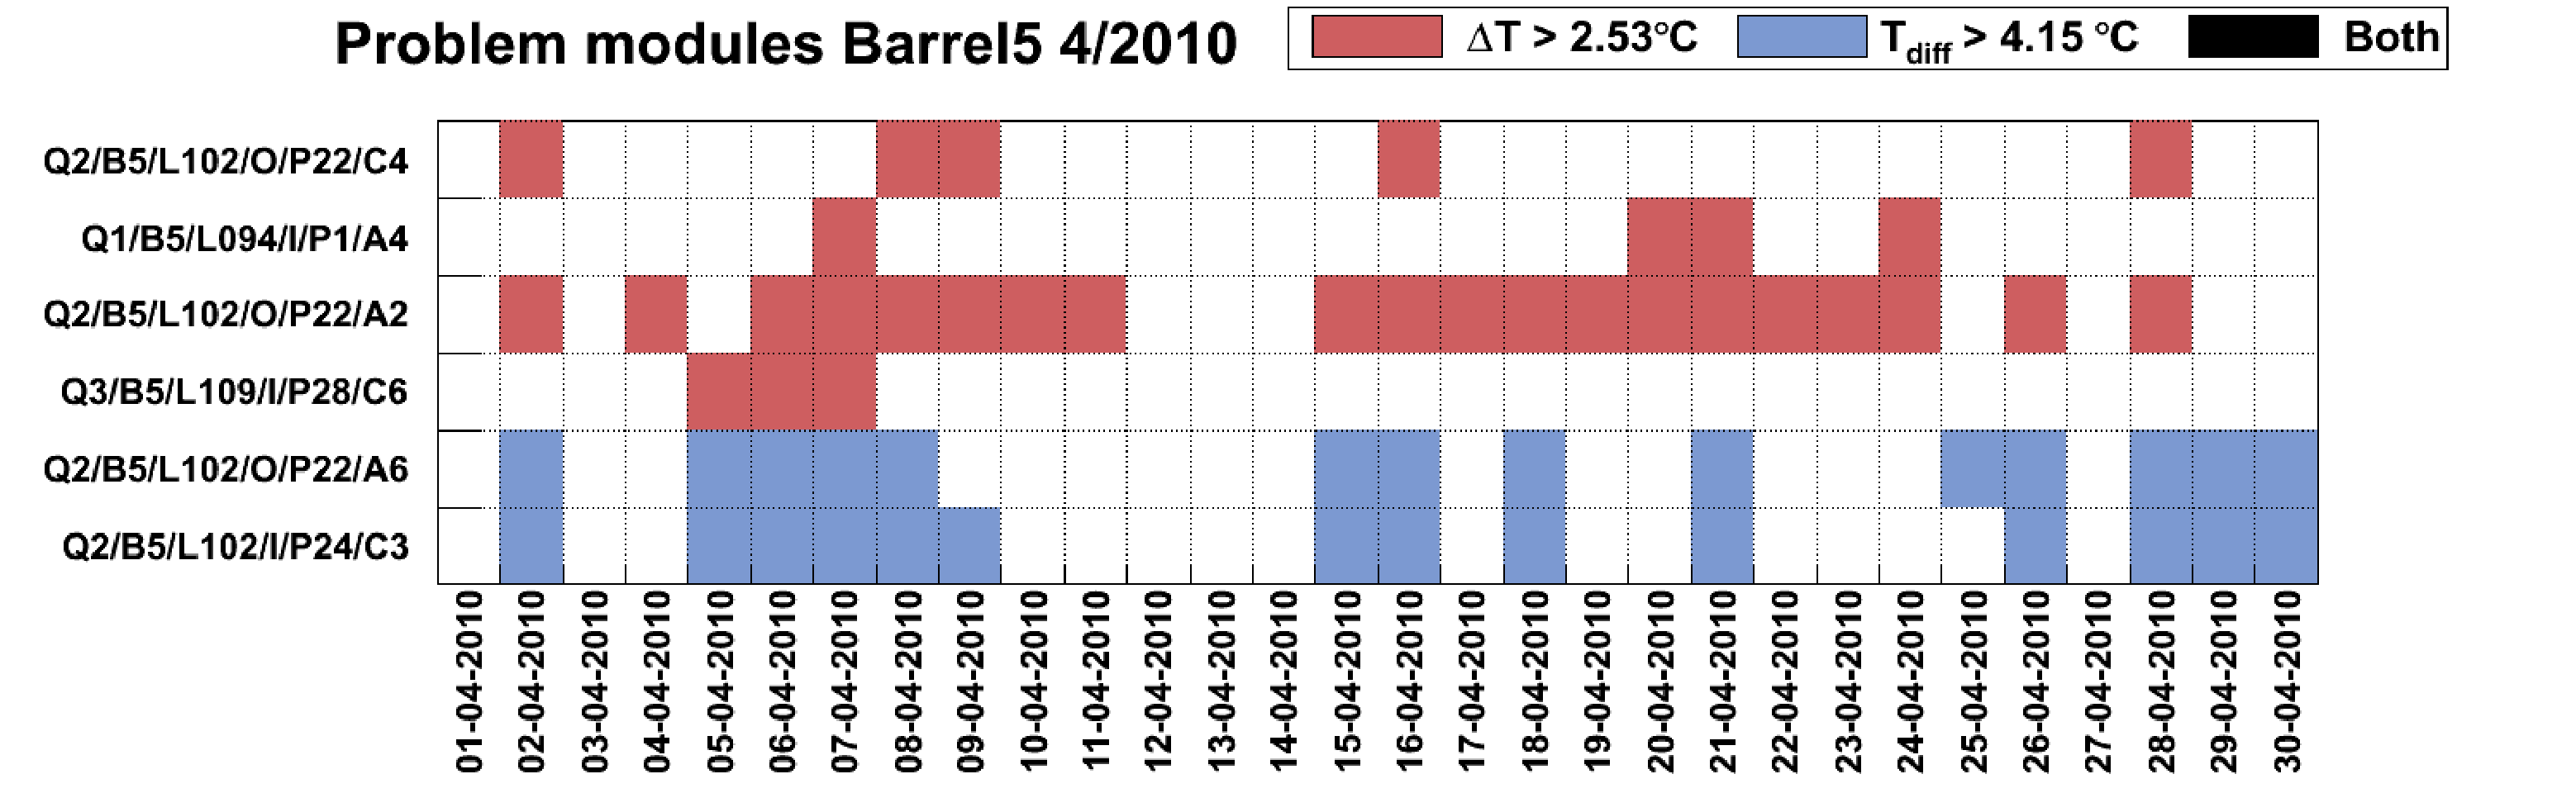
\includegraphics[width=\textwidth]{042010_Barrel5}
	}

	\caption{Problem modules on barrel 5 in April 2010.}
	\label{fig:pm_april}
\end{figure}
 
Of obvious concern is whether the number of problematic modules is increasing.
Figure~\ref{fig:num_pm} shows the number of problem modules above the problem
threshold on a given day as a function of time between 20/01/2010 to 16/10/2012
for the \deltat\ and \tdiff\ monitoring variables. For both monitoring
variables, there is no significant increase in the number of problematic
variables observed as a function of time. Fitting the distributions to a
linear function, the average number of \tdiff\ modules above the problem
threshold is found to increase at a rate of \NumHighTdiffModulesIncreaseRate\
per year. The average number of \deltat\ modules above the problem threshold
is found to increase at a rate of \NumHighDeltaTModulesIncreaseRate\ per year.

\begin{figure}
	\centering
	\subfigure[]{
		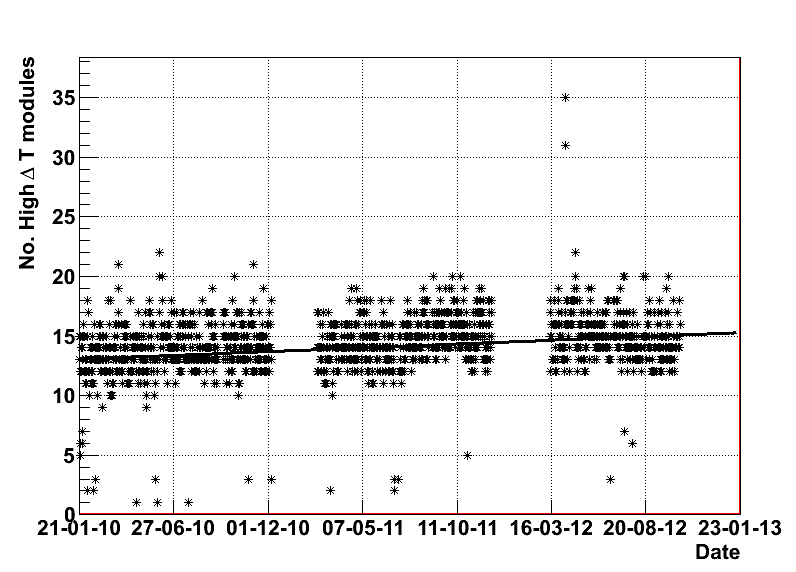
\includegraphics[width=0.47\textwidth]{num_problem_modules/num_high_delta_t}

	}
	\subfigure[]{
		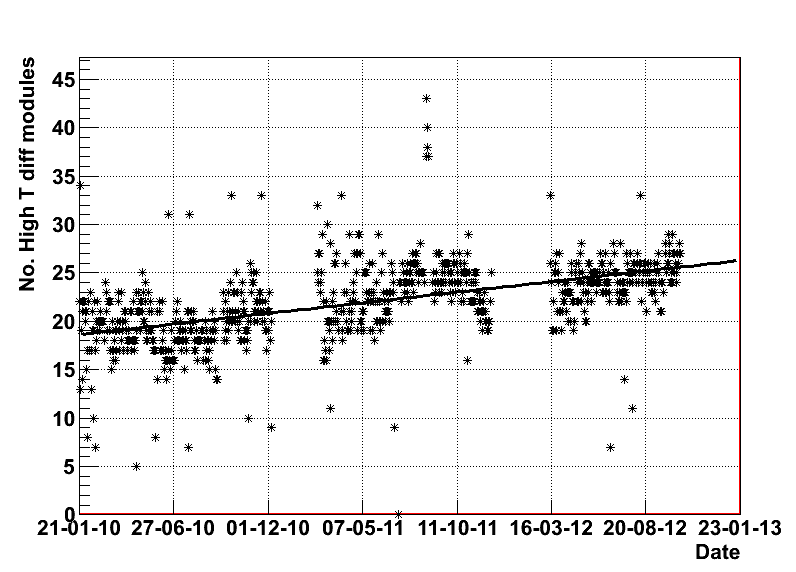
\includegraphics[width=0.47\textwidth]{num_problem_modules/num_high_t_diff}
	}
  \caption[The number of `problematic' modules with (a) \deltat\ and (b) \tdiff\
  with magnitude greater than the problem threshold per day as a function of time
  between 20/01/2010 to 16/10/2012. ]{The number of `problematic' modules with
  (a) \deltat\ and (b) \tdiff\ of greater magnitude than the problem threshold
  per day as a function of time between 20/01/2010 to 16/10/2012. The number of
  `problematic' modules is not seen to increase significantly as a function of
  time.}
	\label{fig:num_pm}
\end{figure}

\section{Behaviour of problematic modules}

For each of the modules identified as problematic at least five times, the value of the problematic monitoring
variable has been plotted as a function of time for the first six months of 2010
in order to identify any trends. For most of the
problematic modules the magnitude of the monitoring variable does not increase
over the period, aside from small fluctuations.  However, one module has been
identified with a high \deltat\ of increasing magnitude, and four modules with a
\tdiff\ of increasing magnitude. A further two show unusual behavior. 

\begin{figure}[h]
 	\centering
	\subfigure[]{
		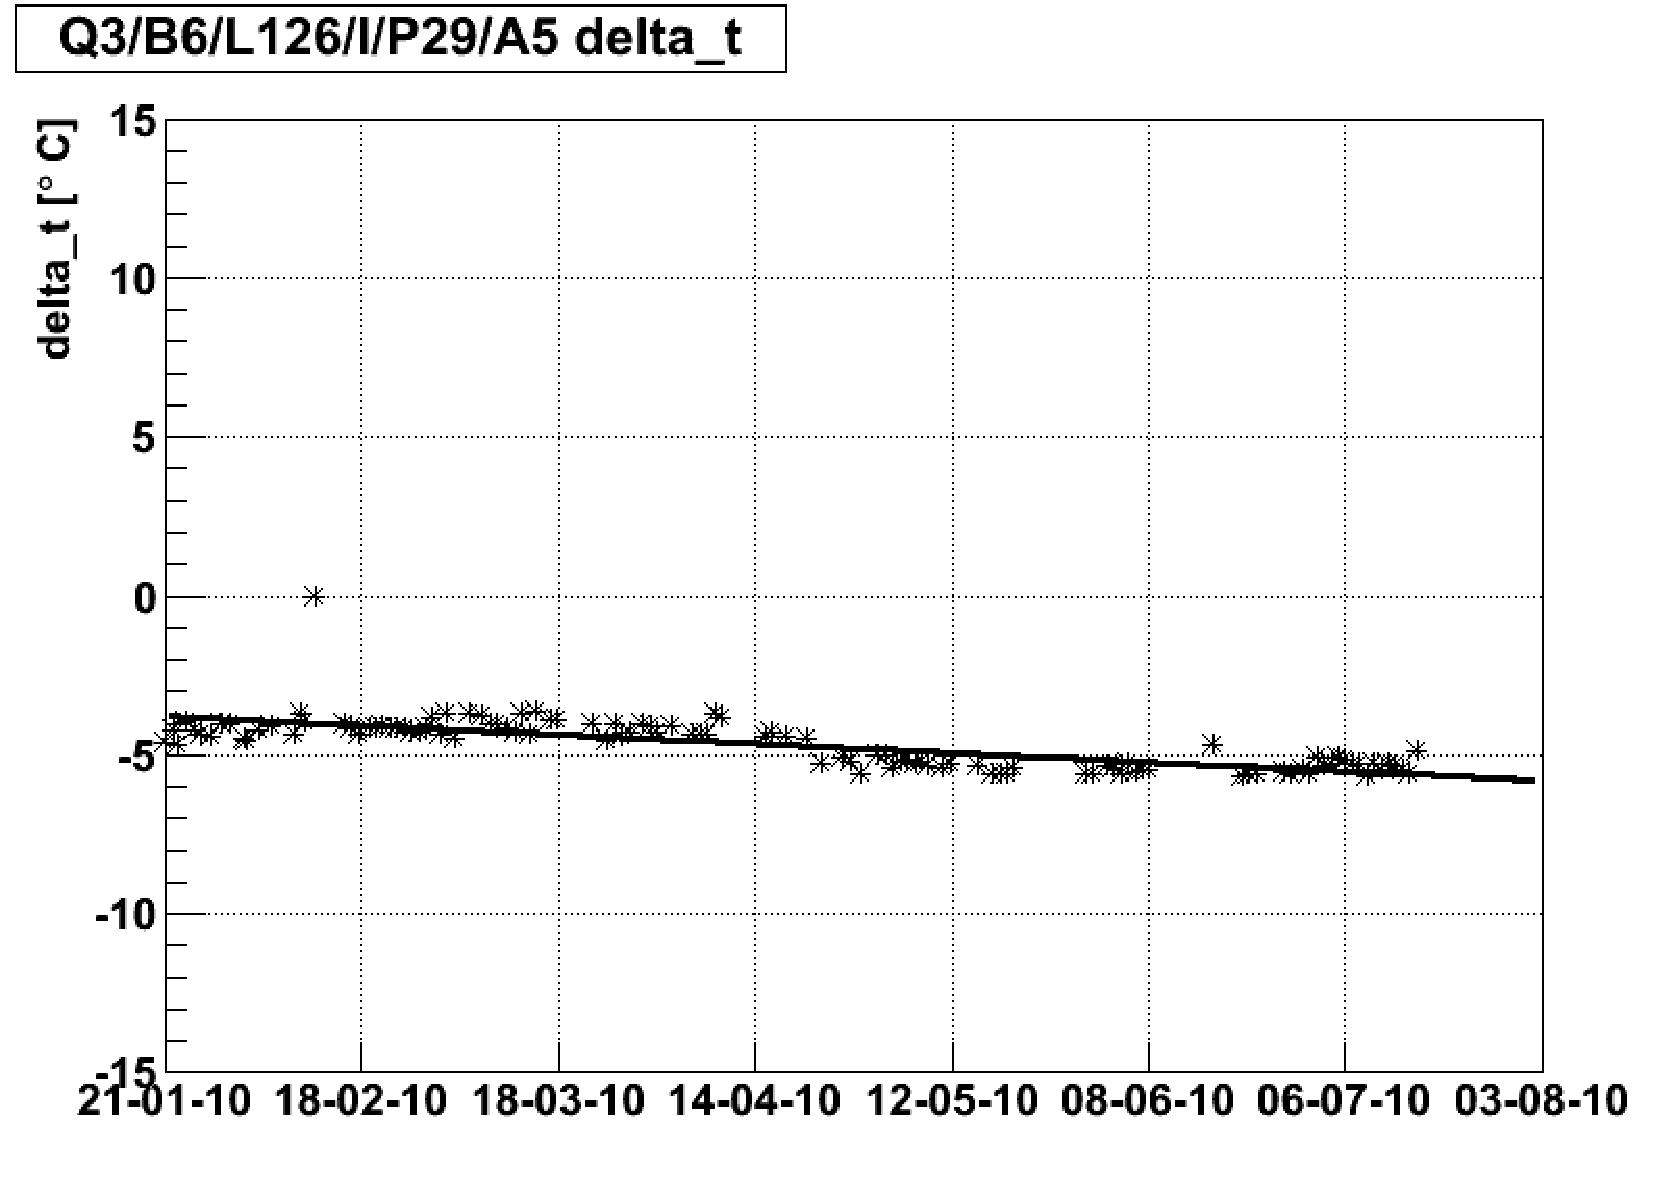
\includegraphics[width=0.47\textwidth]{pm_ev_dt_126-A5}
	}
	\subfigure[]{
		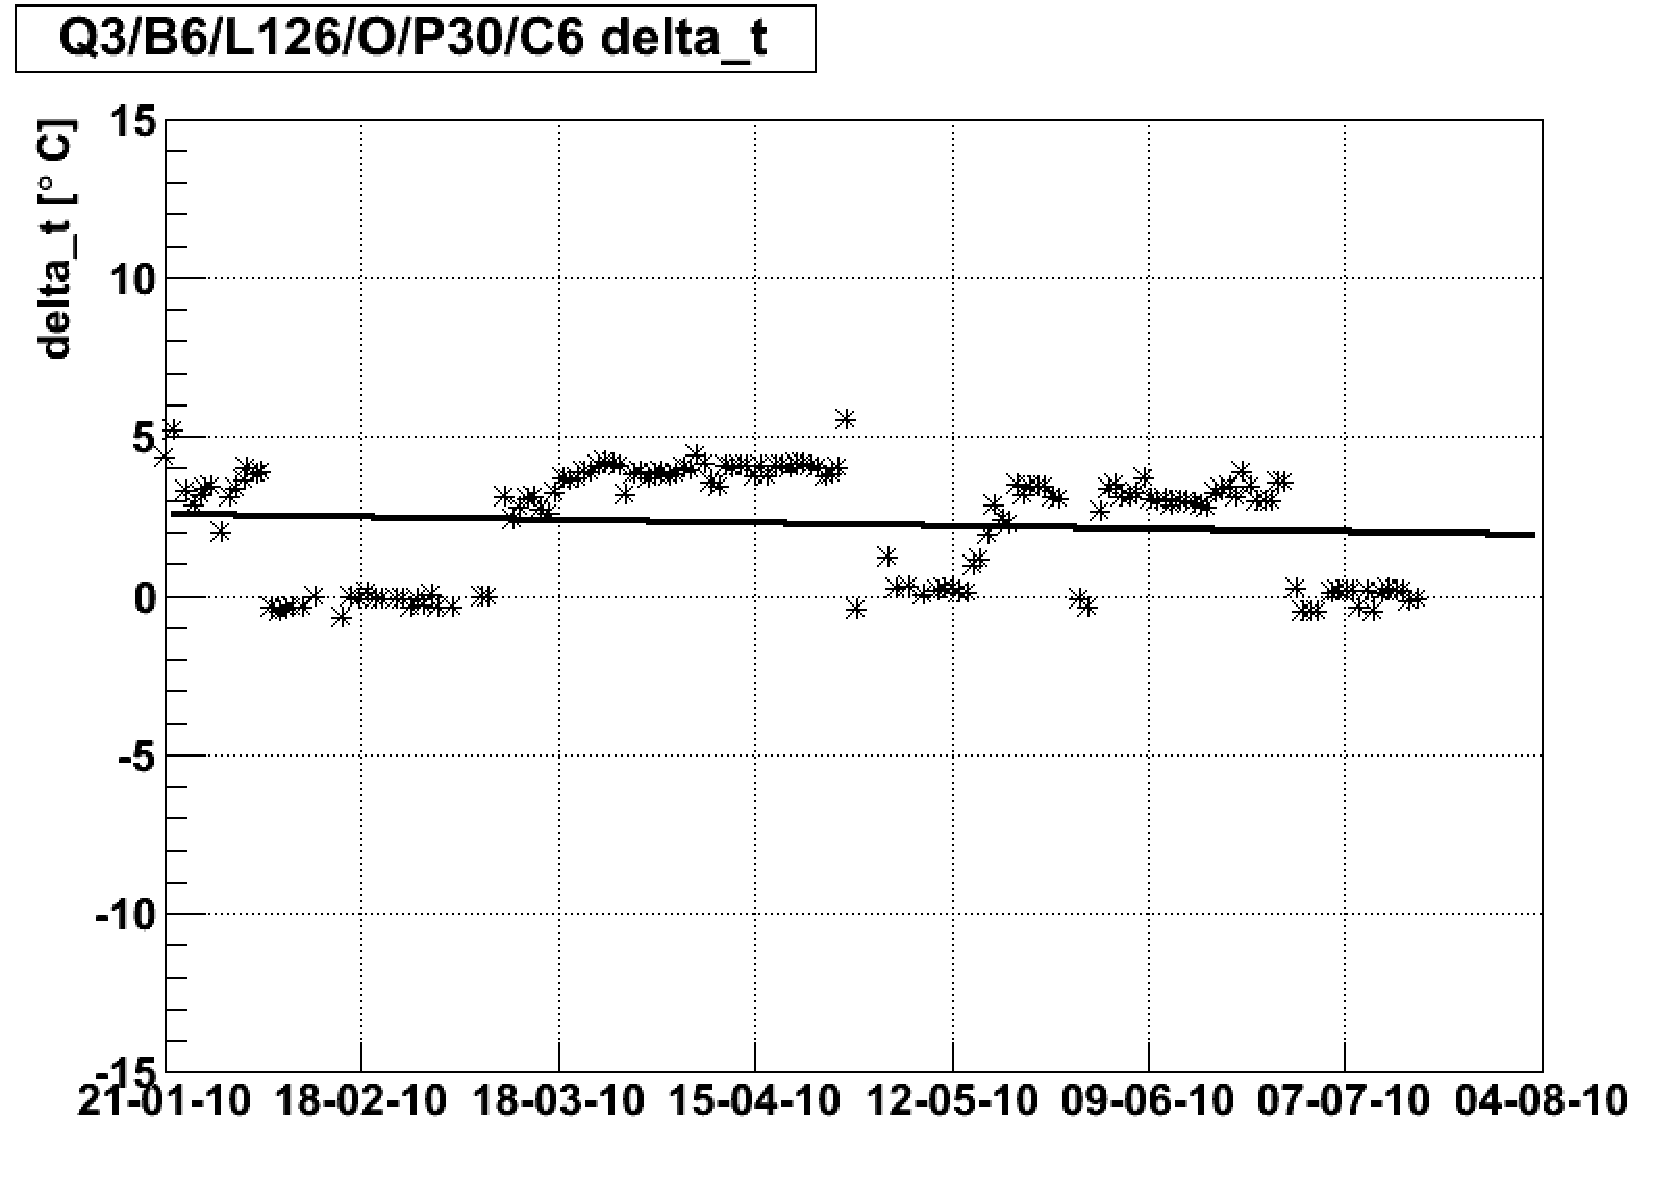
\includegraphics[width=0.47\textwidth]{pm_ev_dt_126-C6}
	}
  \caption{The temperature difference between the front and back of the module
  (\deltat) for (a) barrel module Q3/B6/L126/I/P29/A5 and (b) barrel module
  Q3/B6/L126/O/P30/C6 as a function of time between 20/1/2010 to
  18/7/2010.}
	\label{fig:pm_ev_dt}
\end{figure}

The plot on the left of~\ref{fig:pm_ev_dt} shows the only module with a \deltat\
of increasing magnitude. The temperature difference between the front and back
of the module has increased by about 1.5$^\circ$C in six months, with back of
the module warmer than the front, suggesting worsening thermal coupling across
the module. The plot on the right of~\ref{fig:pm_ev_dt} shows a
module for which \deltat\ jumps between 0\dc\ and 3-4\dc\ every 1 or 2 months.
This suggests an intermittent failure in the integrity of the module. No other problems
with this module have been recorded.

Three modules were observed to have a \tdiff\ becoming more negative with time,
indicating that they are becoming warmer relative to their neighbours by about
1\dc\ over six months. This suggests a failure in coupling to the cooling pipe
that is getting worse with time. One of these modules is shown on the left of
Figure~\ref{fig:pm_ev_tdiff}.  The right hand plot of
Figure~\ref{fig:pm_ev_tdiff} shows a module with \tdiff\ becoming more positive
over time, and also showing sharp jumps in the variable. An increasing positive
\tdiff\ means the module is cooler than its neighbours, and becoming even more
cooler. This would suggest that the module is running at a lower power, although
it is unclear why this would cause the \tdiff\ to increase over time, nor explain
the sudden jumps. Generally modules running at lower power are detected with the
DAQ (Data Acquisition) software, but no problem has been reported for this
module. A further seven modules with a \tdiff\ which jumps between 0\dc\ and
around +7\dc\ have been observed.  All seven of these modules have other known
problems; either the modules do not receive the high voltage, or there is a
problem with the module communication. These modules are out of configuration,
and data sent from these modules is not used for physics.

\begin{figure}[h]
 	\centering
	\subfigure[]{
		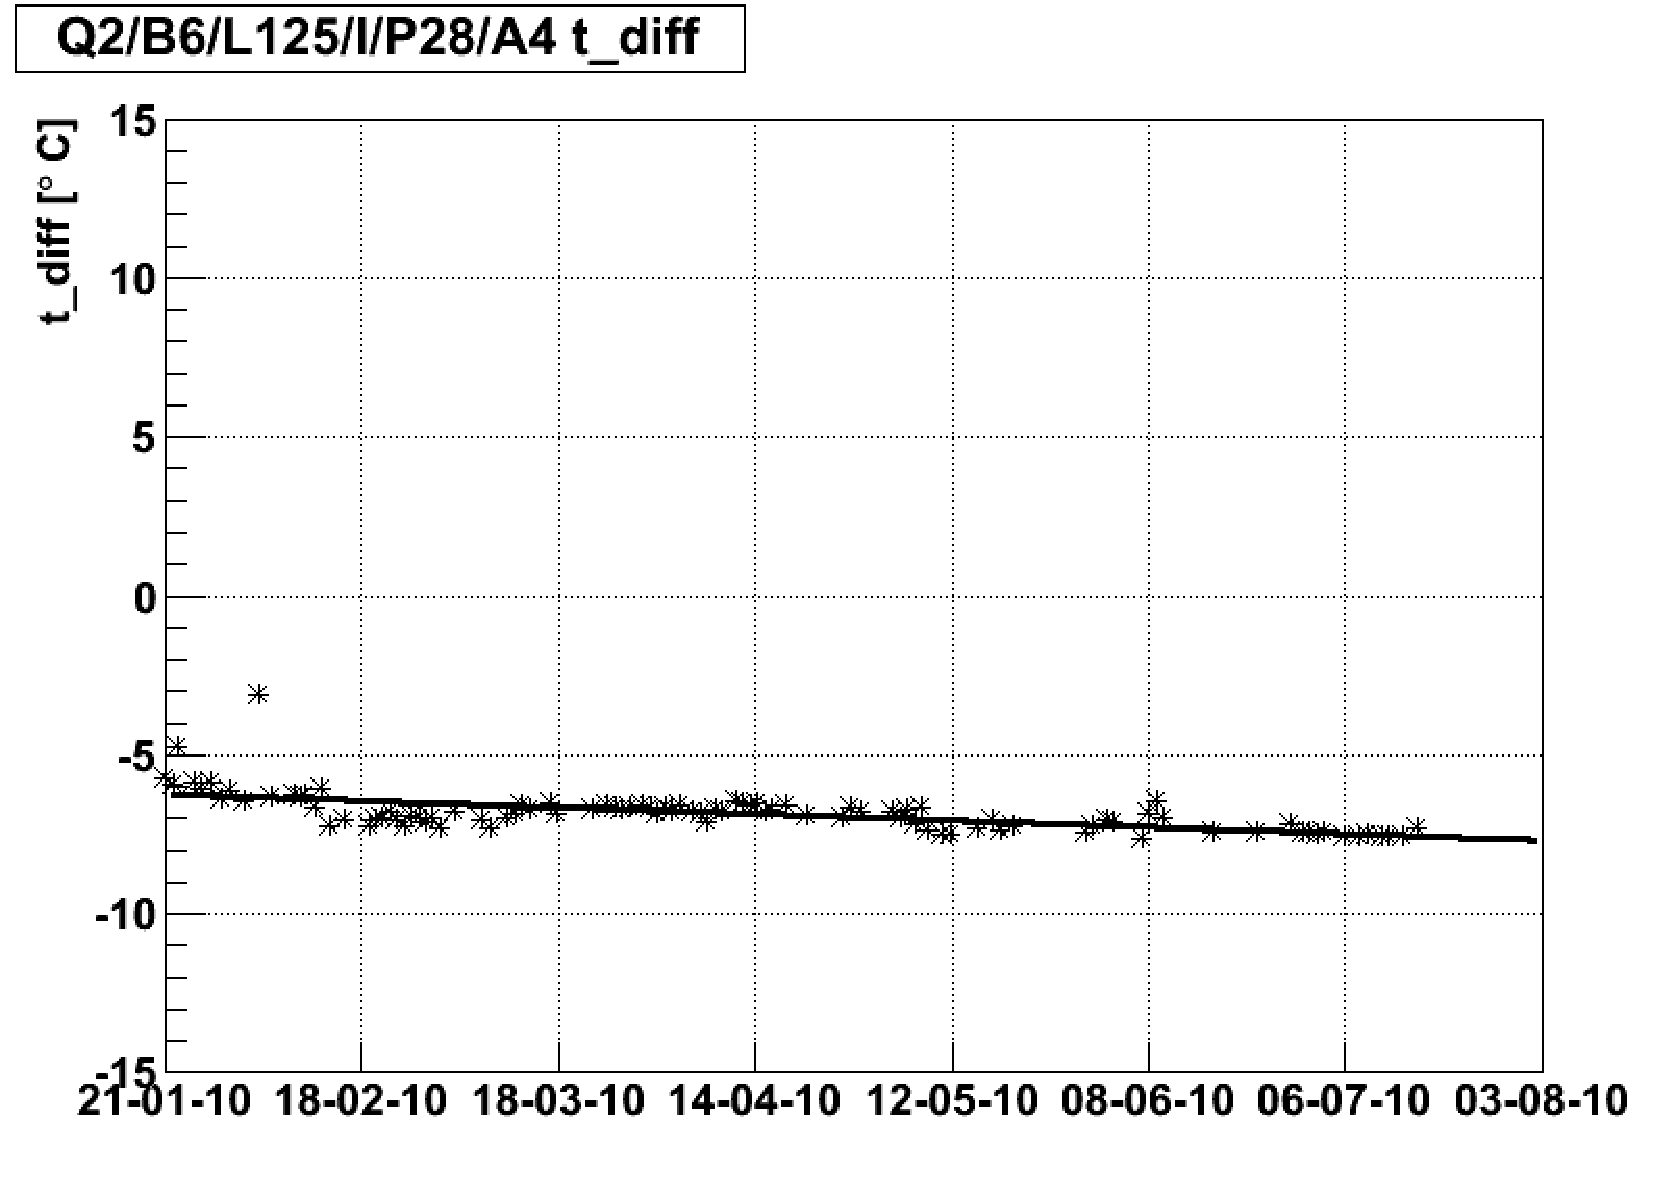
\includegraphics[width=0.47\textwidth]{pm_ev_tdiff_125-A4}
	}
	\subfigure[]{
		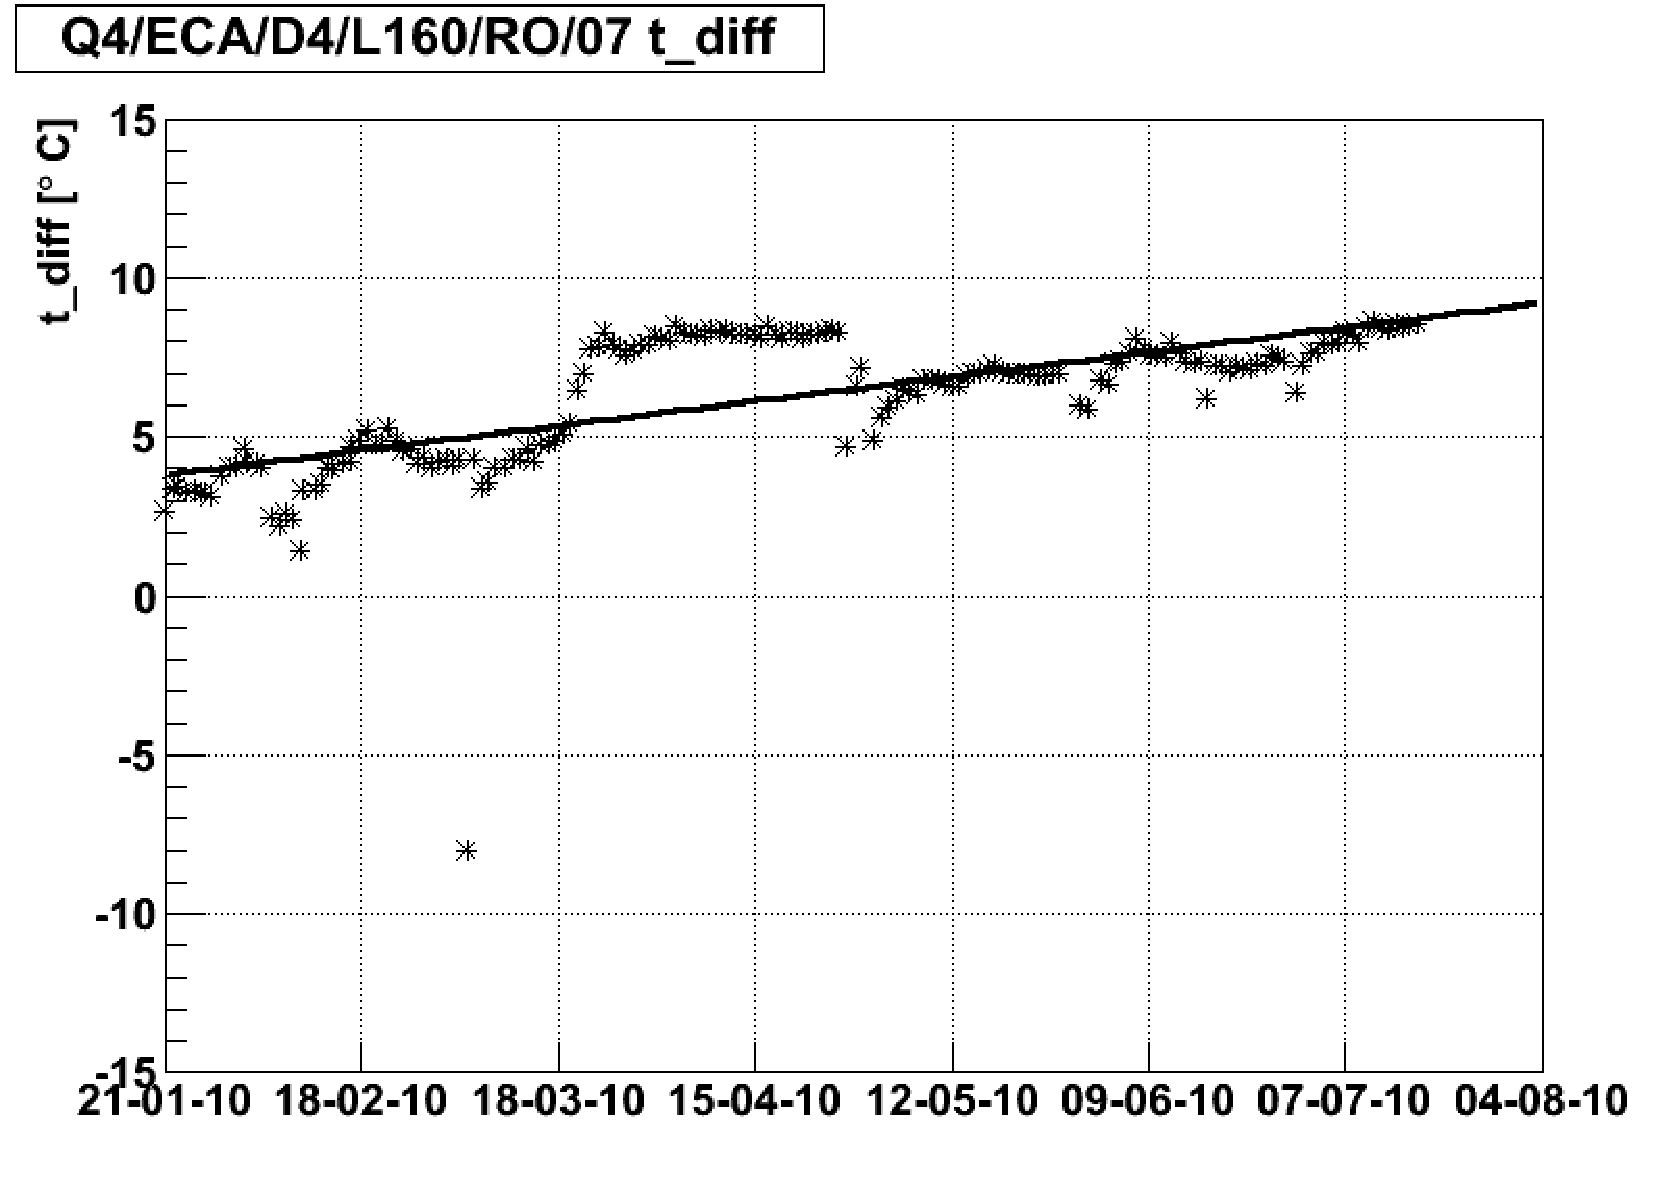
\includegraphics[width=0.47\textwidth]{pm_ev_tdiff_160-07}
	}
	\caption{The difference in temperature between the module and the average
  temperarure of modules on the same cooling structure (\tdiff) as a function of
  time for (a) module Q2/B5/L102/I/P24/C3 and (b) Q4/ECA/D4/L160/RO/07 between
  20/1/2010 and 18/7/2010. }
	\label{fig:pm_ev_tdiff}
\end{figure}

\section{Long Term Trends in Monitoring Variables}

To evaluate the long term performance of the SCT cooling, plots of the mean and
width of the distributions of the monitoring variables as a function of time
were
produced. Such plots allow identification of trends common to all
modules, which would not be identified by the procedure of identifying
`problematic' outliers as described in the previous sections.

\fig{sigma-evo-deltat} shows the width and mean of the \deltat\
distributions as a function of time. For the widths, each point on the graph corresponds to the
width of the Gaussian fit to the \deltat\ distribution for one stable period (such the distribution shown
in~\fig{dt_dist});
similarly for the means, each point corresponds to the mean of the Gaussian fit
for one stable period. The mean and width of the distributions are seen to be
stable as a function of time, indicating that there is no long term shift in the
front-back temperature difference common to all barrel modules. 

\begin{figure}[h]
 	\centering
	\subfigure[]{
		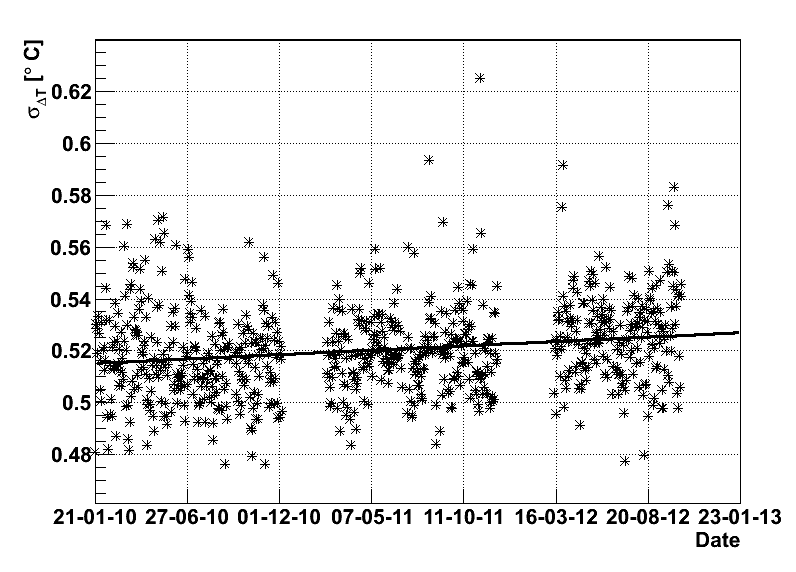
\includegraphics[width=0.47\textwidth]{sigma_evo/SigmaEvolution_delta_t_AllBarrels}
	}
	\subfigure[]{
		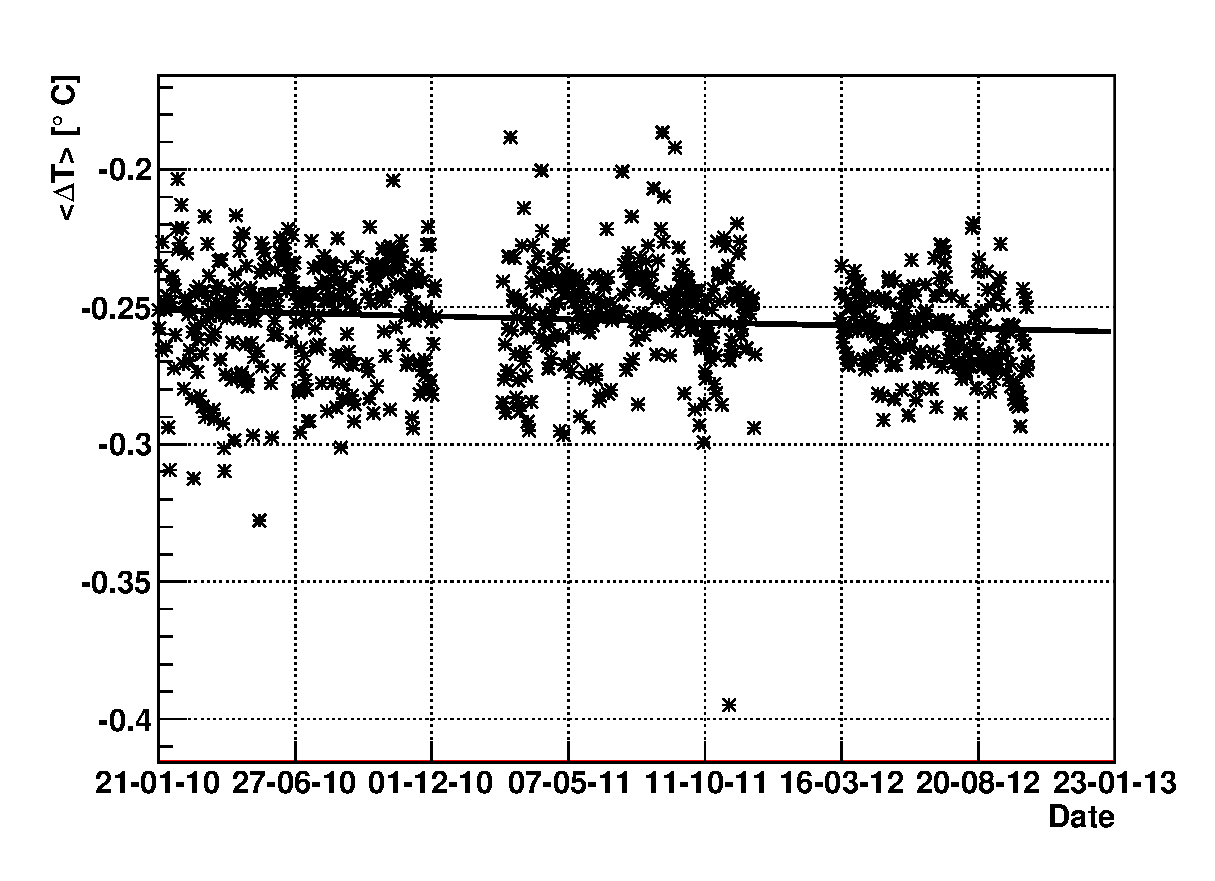
\includegraphics[width=0.47\textwidth]{sigma_evo/MeanEvolution_delta_t_AllBarrels}
	}
  \caption{The (a) width and (b) mean of the module \deltat\ distribution for SCT
  barrel modules as a function of time.}
	\label{fig:sigma-evo-deltat}
\end{figure}

\fig{sigma-evo-tavg} shows the width and mean of the module temperature
distributions as a function of time. Similarly to the \deltat\ plots, each point
on the graph corresponds to the width or mean of the Gaussian fit to the module
temperature distributions for one stable period. For barrel modules, the
temperature is taken as the average of the front and back thermistor
temperatures. The mean of the temperature distributions are observed to increase
slightly as a function of time; this is attributed to increasing occupancy as
the instantaneous luminosity increased, which causes increased power dissipation
in the readout chips. The slight decrease in temperature at the start of the
2012 run is attributed to calibration work occurring during the recommissioning,
and the sudden jump in the average endcap module temperature near the start of
2010 is due to the changing of one of the compressors.  The width of the
temperature distributions are observed to be
stable as a function of time.

\fig{sigma-evo-tdiff} shows the width of the \tdiff\
distributions as a function of time; the means are not shown as they are
identically zero by construction. The widths are observed to be stable, indicating
that there is no long term increase in the spread of module temperatures for
modules along a cooling pipe.

\begin{figure}[h]
 	\centering
	\subfigure[Barrels]{
		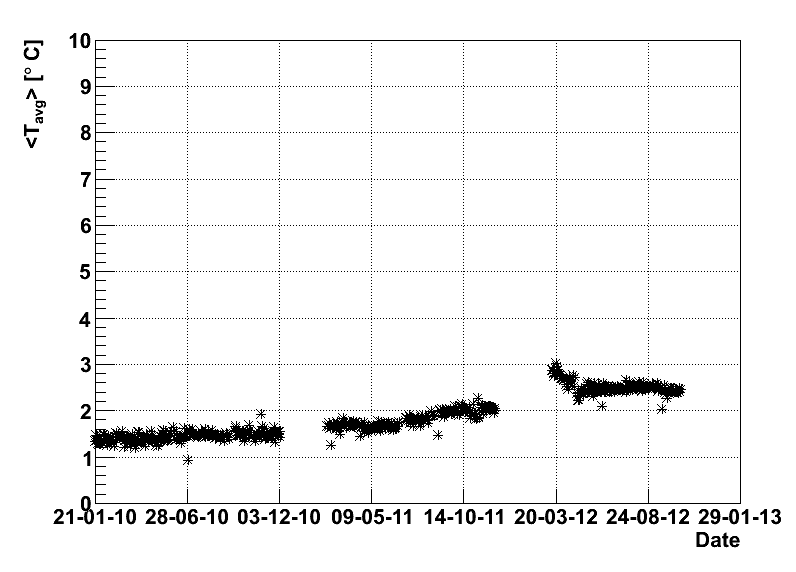
\includegraphics[width=0.47\textwidth]{sigma_evo/MeanEvolution_t_avg_AllBarrels}
	}
	\subfigure[Endcaps]{
		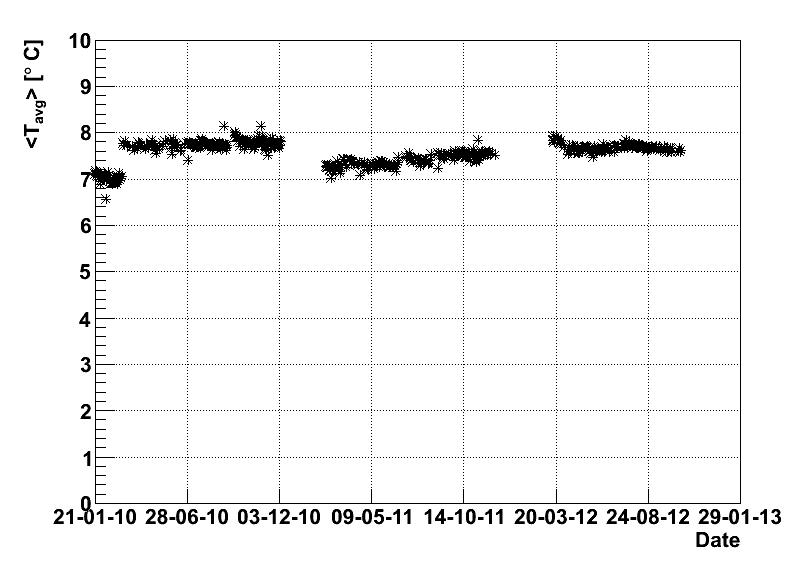
\includegraphics[width=0.47\textwidth]{sigma_evo/MeanEvolution_t_avg_Endcaps}
  }
	\subfigure[Barrels]{
		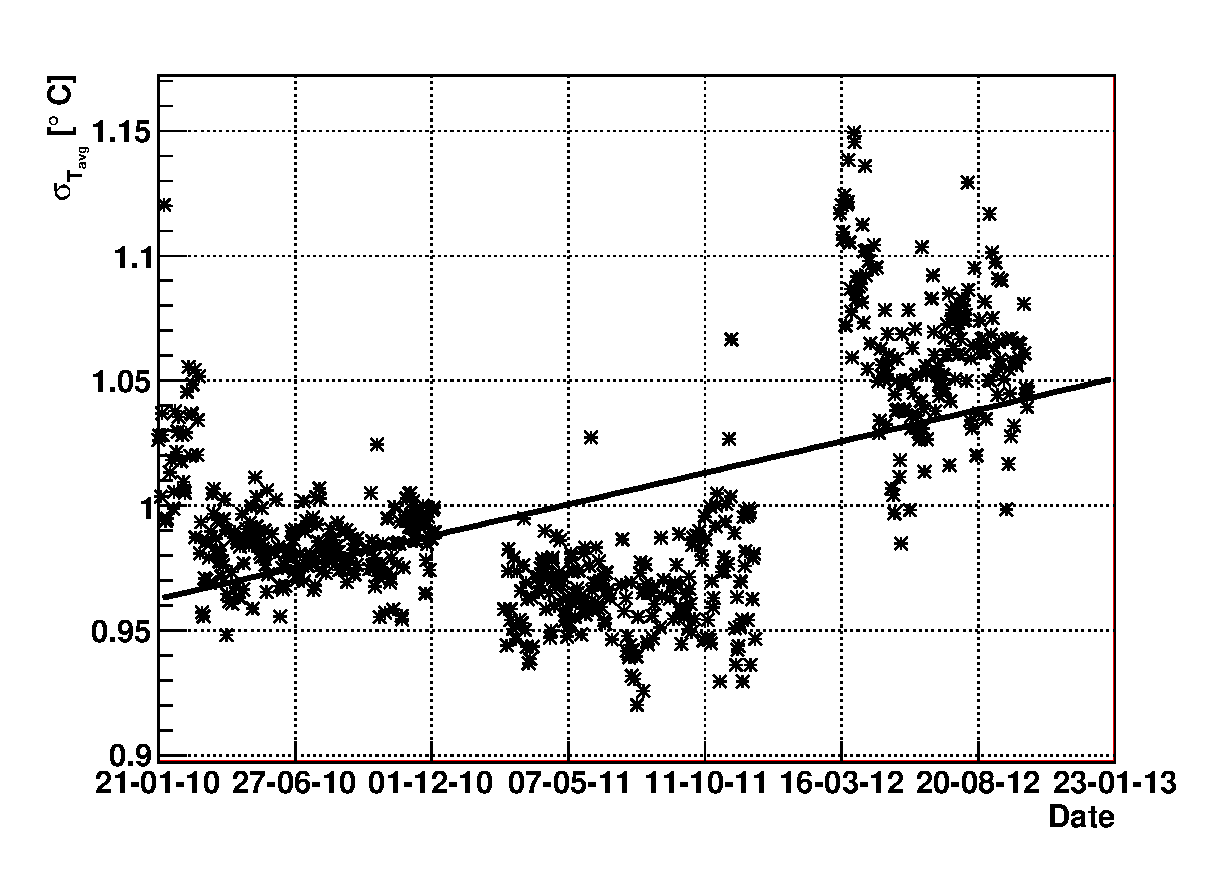
\includegraphics[width=0.47\textwidth]{sigma_evo/SigmaEvolution_t_avg_AllBarrels}
	}
	\subfigure[Endcaps]{
		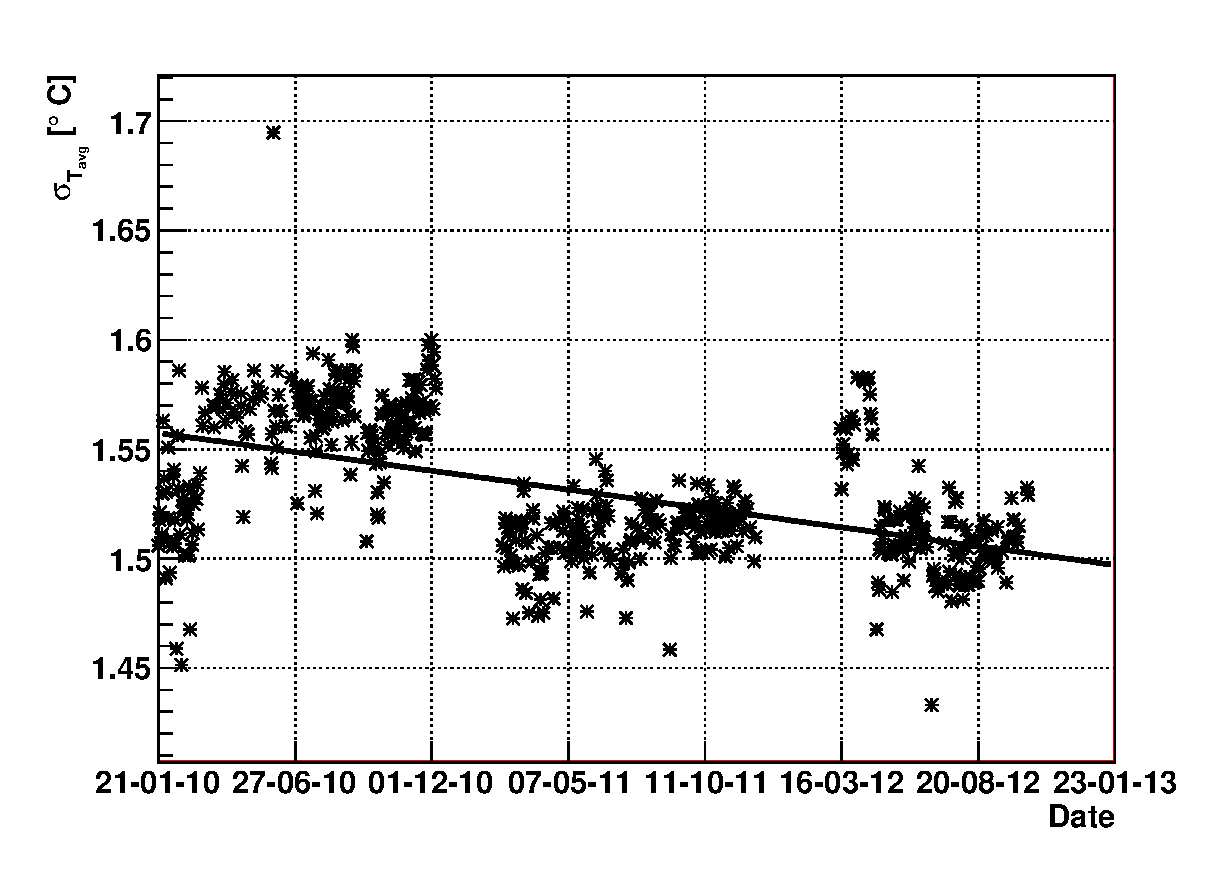
\includegraphics[width=0.47\textwidth]{sigma_evo/SigmaEvolution_t_avg_Endcaps}
  }
  \caption{Figures (a) and (b) show the mean of the module temperature
  distribution as a function of time for the SCT barrels and encaps,
  respectively. Figures (c) and (d) show the width of the module temperature
  distribution as a function of time, again for the barrels and endcaps
  respectively.}
	\label{fig:sigma-evo-tdiff}
\end{figure}

\begin{figure}[h]
 	\centering
	\subfigure[Barrels]{
		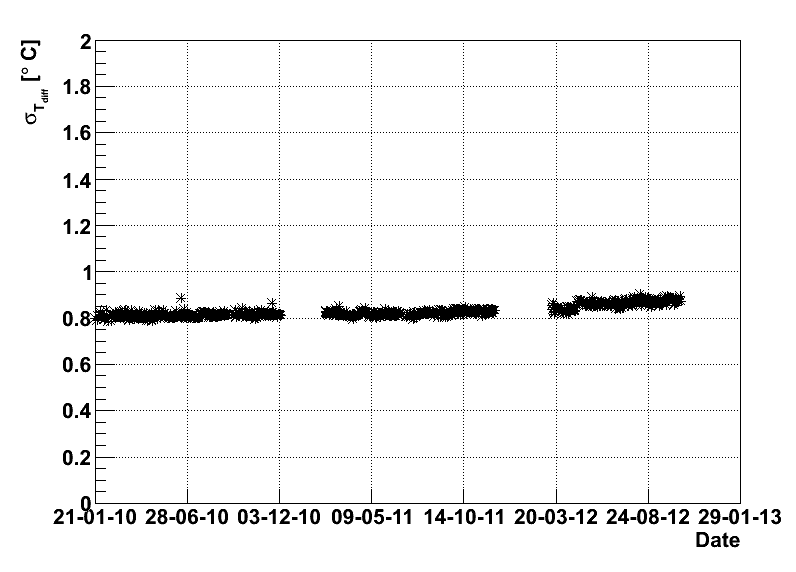
\includegraphics[width=0.47\textwidth]{sigma_evo/SigmaEvolution_t_diff_AllBarrels}
	}
	\subfigure[Endcaps]{
		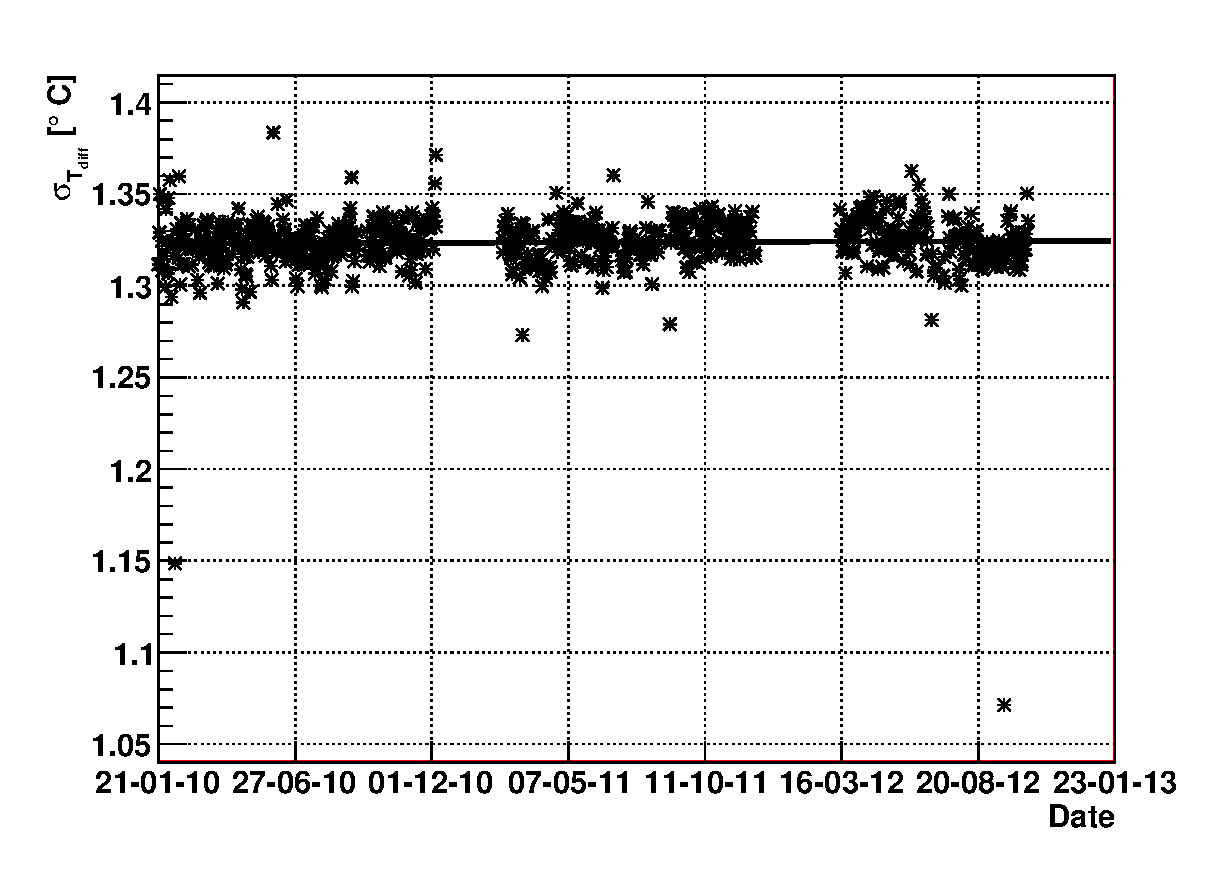
\includegraphics[width=0.47\textwidth]{sigma_evo/SigmaEvolution_t_diff_Endcaps}
  }
  \caption{The width of the \tdiff\ distribution as a function of time for (a)
  the barrels and (b) the endcaps.}
	\label{fig:sigma-evo-tavg}
\end{figure}

\section{Conclusions}

Studies of the performance of the SCT cooling system have been performed. 
Variables for identifying modules
loosing coupling to the cooling pipe and for identifying modules loosing
mechanical integrity have been defined, and an automated monitoring set up to
produce plots of the distributions of these variables and to
identify `problematic' modules. Only a small fraction of the modules are found
to be problematic, and in  most cases these problematic modules are known to have other
problems and their readout is not used for physics analysis. Over almost three years of
running the number of problematic modules is not seen to increase significantly,
and the mean and width of the distributions of the monitoring variables remain
stable.

